% !TeX encoding = UTF-8
\documentclass[11pt,a4paper,twoside,svgnames]{article}

%%%%%%%%%%%%%%%%%%%%%%%%%%%%%%%%%%%%%%%%
%%%%%%%%%%%%%%%%%%%%%%%%%%%%%%%%%%%%%%%%
%
% ENCODAGES, LANGUES, AMS ET AUTRES 
%
%%%%%%%%%%%%%%%%%%%%%%%%%%%%%%%%%%%%%%%%
%%%%%%%%%%%%%%%%%%%%%%%%%%%%%%%%%%%%%%%%
%
\usepackage[T1]{fontenc} 
\usepackage[utf8]{inputenc}
\usepackage[english,frenchb]{babel}
%
\frenchbsetup{StandardLists=true} 
\usepackage{enumitem}
\usepackage{xspace}
\usepackage{amssymb,mathtools,pifont} 
\usepackage{xcolor}
\usepackage{graphicx}

%%%%%%%%%%%%%%%%%%%%%%%%%%%%%%%%%%%%%%%%
%%%%%%%%%%%%%%%%%%%%%%%%%%%%%%%%%%%%%%%%
%
% ALGORITHMES ET PSEUDO-CODES
%
%%%%%%%%%%%%%%%%%%%%%%%%%%%%%%%%%%%%%%%%
%%%%%%%%%%%%%%%%%%%%%%%%%%%%%%%%%%%%%%%%
%
\usepackage{algorithm}
\usepackage[noend]{algpseudocode}
%
\floatname{algorithm}{Algorithme}
\algrenewcommand\algorithmicrequire{\textbf{Données :}}
\algrenewcommand\algorithmicensure{\textbf{Résultat :}}
%
\algnewcommand\algorithmicto{\textbf{to}}
\algrenewtext{For}[3]{\algorithmicfor\ #1 $\gets$ #2 \algorithmicto\ #3 \algorithmicdo}
%
\algrenewcommand{\algorithmiccomment}[1]{\hfill{\color{Green}$\triangleright$ #1}}

%%%%%%%%%%%%%%%%%%%%%%%%%%%%%%%%%%%%%%%%
%%%%%%%%%%%%%%%%%%%%%%%%%%%%%%%%%%%%%%%%
%
% MARGES, ENTÊTES ET PIEDS DE PAGE, TITRE
%
%%%%%%%%%%%%%%%%%%%%%%%%%%%%%%%%%%%%%%%%
%%%%%%%%%%%%%%%%%%%%%%%%%%%%%%%%%%%%%%%%
%
\usepackage[hcentering=true,nomarginpar,textwidth=426.8pt,textheight=650.2pt,headheight=24pt]{geometry}
%
\usepackage{fancyhdr}
\fancypagestyle{plain}{
	\fancyhf{}
	\renewcommand{\headrulewidth}{0pt}
	\renewcommand{\footrulewidth}{0pt}}
\pagestyle{fancy}
	\fancyhf{}
	\fancyhead[LO]{MCR -- Printemps 2017}
	\fancyhead[RO,LE]{\thepage}
	\renewcommand{\headrulewidth}{0.4pt}
	\renewcommand{\footrulewidth}{0pt}
%
\usepackage{sectsty}
\allsectionsfont{\color{DarkOrange}}
\title{\color{Chocolate}\huge\bfseries CoRe\\Implémentation du patron\\chaîne de responsabilité}
\author{Antoine \bsc{Friant}\\
Christopher \bsc{Meier}\\
Daniel \bsc{Palumbo}\\
Lawrence \bsc{Stalder}\\
Valentin \bsc{Finini}}
\date{\today}

\begin{document}

\maketitle
\clearpage
\tableofcontents
\clearpage
\section{Introduction}
CoRe est un projet dont l'objectif est de démontrer une implémentation du patron de conception "chaîne de responsabilité" dans une application ludique.

\section{Le jeu}
CoRe (pour "Chain of Responsability") est un jeu de type \textit{shoot 'em up} à défilement horizontal. Le joueur pilote un vaisseau qui avance à vitesse constante vers la droite, tandis que des obstacles à éviter viennent dans le sens opposé. Le joueur peut tirer des projectiles pour détruire ces obstacles.\\

Pour tirer un projectile, il faut appuyer sur les touches J, K ou L. Chacune de ces touches tirent une couleur différente, et il est possible des mélanger ces couleurs pour en créer de nouvelles. Les trois couleurs à la fois produisent du noir.\\

Afin de détruire un astéroïde, il faut tirer dessus avec la couleur qui lui correspond. S'il explose, une réaction en chaîne (gérée par le patron chaîne de responsabilité) est déclenchée. Dans ce cas, l'objet le plus proche est lui aussi touché par la même couleur. Il peut alors exploser à son tour, et ainsi de suite ...\\

Afin de détruire un bloc de glace, il faut qu'il soit touché par une réaction en chaîne de n'importe quelle couleur. Tirer dessus directement n'a pas d'effet. Lorsqu'il explose, il transforme la couleur reçue en blanc avant de continuer la réaction en chaîne. Le blanc détruit les astéroïdes de n'importe quelle couleur, ce qui a pour effet de faire exploser tous les astéroïdes de l'écran.\\

Les satellites ne réagissent que lorsqu'ils reçoivent du noir, lançant deux réactions en chaîne de couleur aléatoire (une chaude et une froide) en direction de l'objet le plus proche. Ils explosent après avoir reçu 20 tirs noirs.\\

Afin de ne pas rendre les réactions en chaîne trop rares, il a été décidé de faire en sorte que les astéroïdes apparaissent par groupe de couleur chaudes ou froides. Il y a donc plus de chance d'avoir deux objets adjacents de la même couleur que si leur couleur était parfaitement aléatoire. La difficulté du jeu croît à mesure que le temps passe (de plus en plus d'obstacles apparaissent), et un score est affiché comme indicateur de la performance du joueur.

\section{Implémentation}
\subsection{Libgdx}
Libgdx\footnote{https://libgdx.badlogicgames.com/} est un ensemble de librairies open-source et sous licence Apache 2.0. Il forme un framework minimaliste qui n'impose quasiment aucune structure ou classe au programmeur. Si le projet est correctement configuré, il est possible d'exécuter la même application sur desktop, IOS, Android et navigateur (HTML5).\\

Dans le cas de CoRe, il n'y a qu'une seule plateforme ciblée : desktop. La classe DesktopLauncher contient la méthode main, ainsi que les configurations de base pour lancer l'application (taille et titre de base de la fenêtre, par exemple). La boucle d'exécution est alors lancée.\\

La classe CoR (dont le nom est laissé au choix du développeur) contient la boucle d'exécution du jeu. La méthode create est appelée au démarrage, puis la méthode render est appelée à chaque rendu d'un image du jeu (60 fois par seconde par défaut). La méthode dispose est appelée à la fermeture du programme. Le développeur est libre de faire ce qu'il veut dans le corps de ces méthodes.

\subsection{Structure générale}
structure générale
justifier la duplication de code

\clearpage
\section{Diagramme de classes}
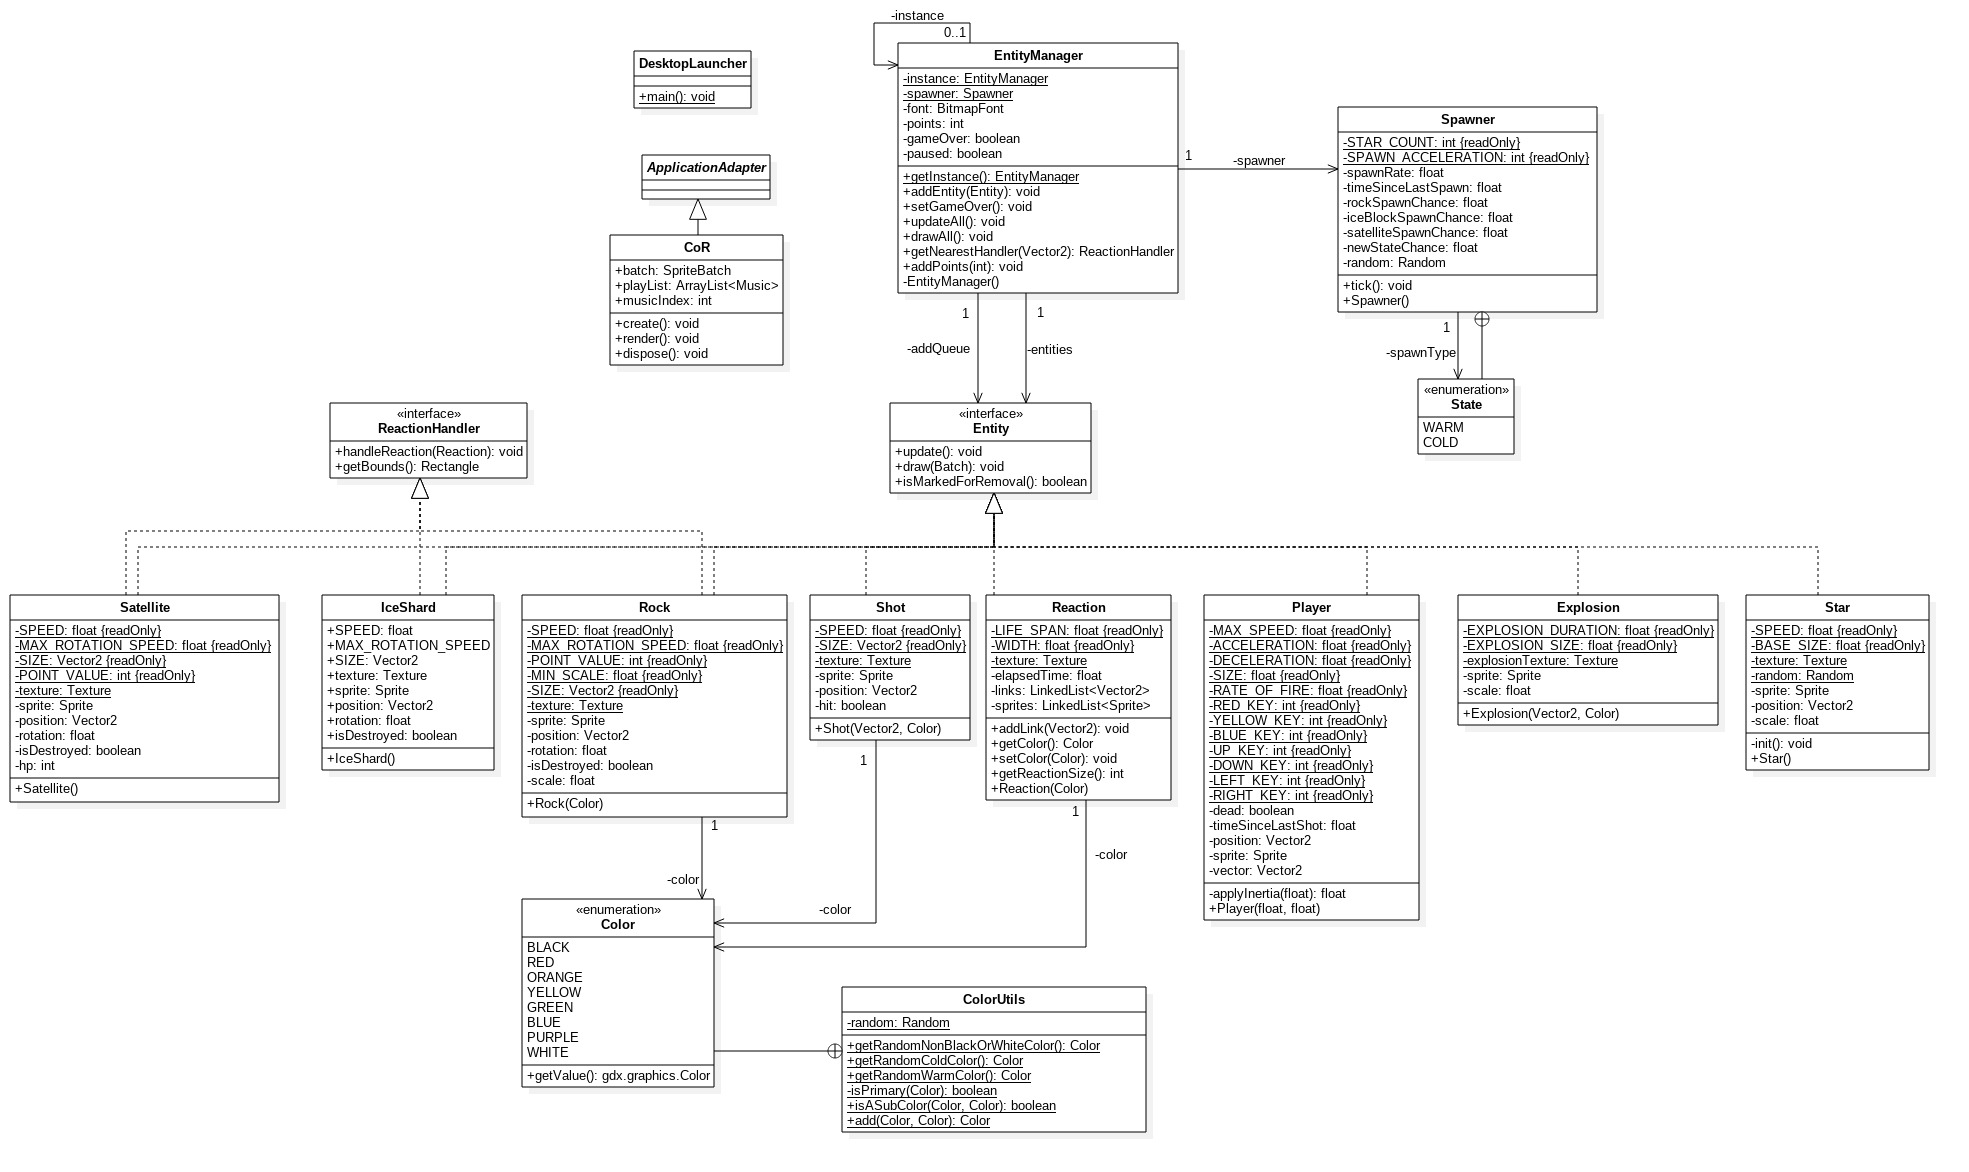
\includegraphics[scale=0.35,angle=90,origin=c]{uml_cor.jpg}
\clearpage
\section{Patrons de conception}
\subsection{Chaîne de responsabilité}

\subsection{Singleton}
EntityManager
\subsection{Classe utilitaire}
ColorUtils : Abstraction de Color et mélanges/génération de couleur.

\section{Conclusion}

\end{document}
